\chapter{Motivation}

Prototyping, design evaluation, and the measurement of physical properties in experiments make a daily occurrence in the engineering praxis. Those tasks often involve the generation and sampling of electrical signals coming to and from sensors, actuators, and other circuitry. 

In the recent years, a wide range of intelligent sensors became available thanks to the drive for miniaturization in the consumer electronics industry. Those devices often provide sufficient accuracy and precision while keeping the circuit complexity and cost low. In contrast to analog sensors, here the signal conditioning and processing circuits are built into the sensor itself, and we access it using a digital connection.

\begin{figure}[H]
	\centering
	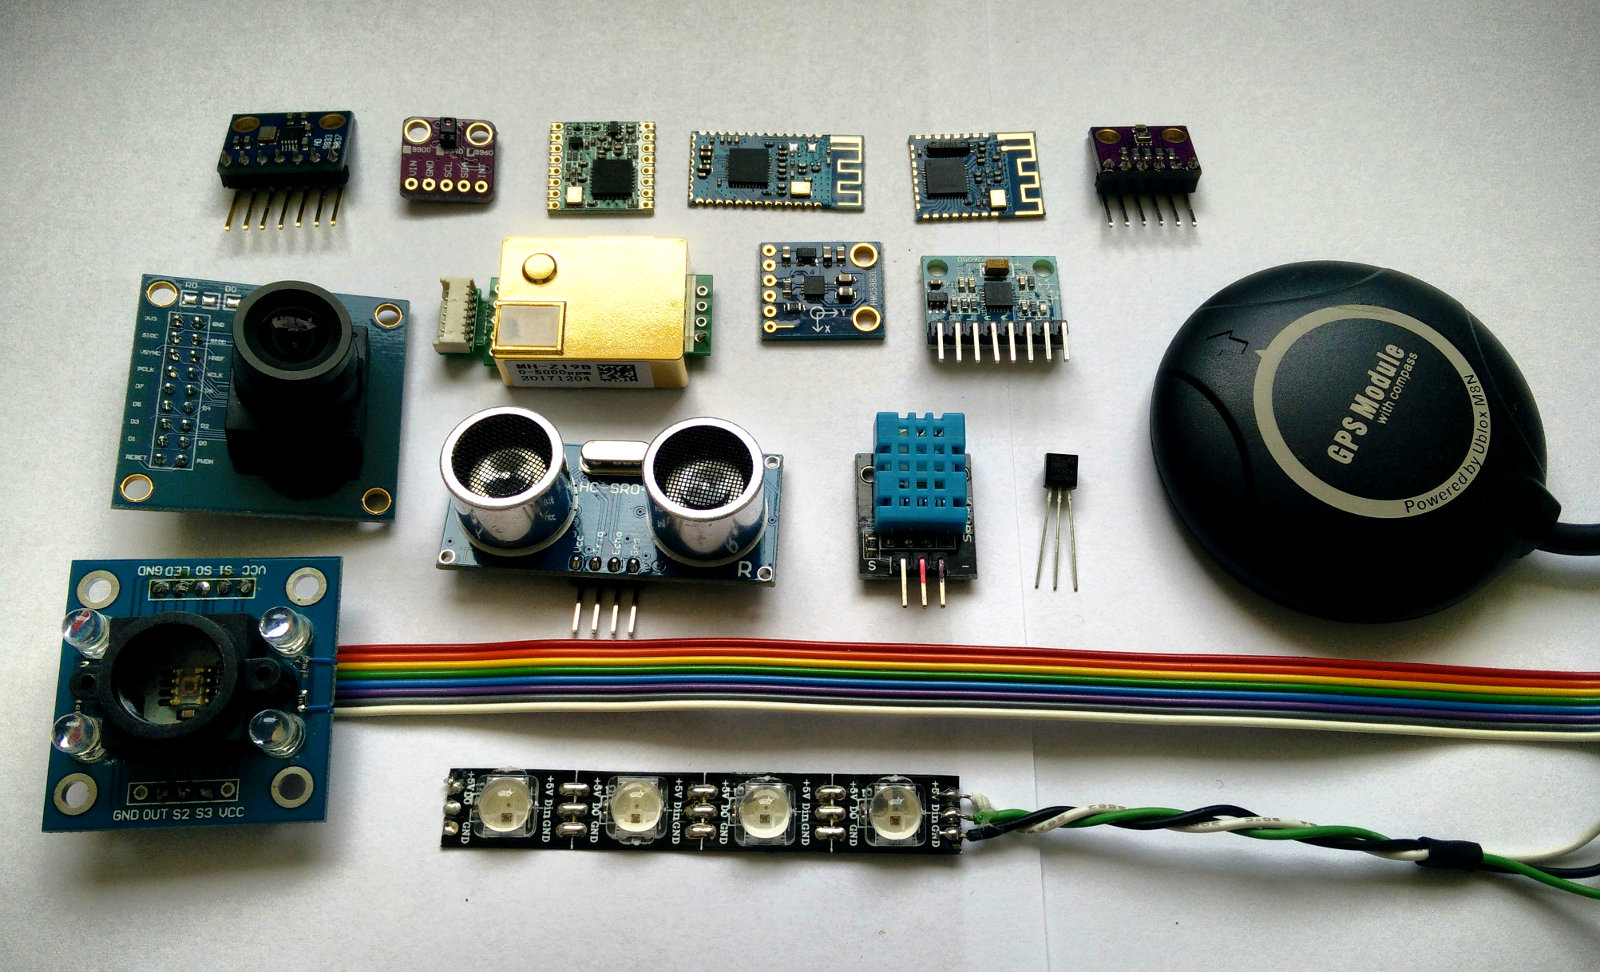
\includegraphics[width=0.8\textwidth] {img/inteligent-sensors.jpg}
	\caption[A collection of intelligent sensors and devices]{A collection of intelligent sensors and devices, most on breadboard adapters: (from top left) a waveform generator, a gesture detector, a LoRa and two Bluetooth modules, an air quality and pressure sensor, a CO$_2$ sensor, a digital compass, an accelerometer, a GPS module, a camera, an ultrasonic range finder, a humidity sensor, a 1-Wire thermometer, a color detector and an RGB LED strip.}
\end{figure}

To conduct experiments with those integrated modules, or just familiarize ourselves with a device before using it in a project, we need an easy way to interact with them. It is also convenient to have direct access to hardware, be it analog signal sampling, generation, or even just logic level inputs and outputs. However, the drive for miniaturization and the advent of \gls{USB} lead to the disappearance of low-level computer ports, such as the printer port (LPT), that would provide an easy way of doing so.

Today, when one wants to perform measurements using a digital sensor, the usual route is to implement an embedded firmware for a microcontroller that connects to the \gls{PC} through \gls{USB}, or perhaps shows the results on a display. This approach has its advantages, but is time-consuming and requires knowledge entirely unrelated to the measurements we wish to perform. It would be advantageous to have a way to interface hardware without having to burden ourselves with the technicalities of the connection, even at the cost of lower performance compared to a specialized device or a professional tool. 

The design and implementation of such a universal instrument is the object of this work. For technical reasons, such as naming the source code repositories, we need a name for the project; it'll be hereafter called \textit{GEX}, a name originating from ``GPIO Expander''.

\section{The Project's Expected Outcome}\label{sec:expected-outcome}

It has been a desire of the author for many years to create a universal instrument connecting low-level hardware to a computer, and, with this project, it is finally being realized. Several related projects approaching this problem from different angles can be found on the internet; those will be presented in chapter~\ref{sec:prior-art}. This project should not end with yet another tinkering tool that will be produced in a few prototypes and then forgotten. By building an extensible, open-source platform, GEX can become the foundation for future projects which others can expand, re-use and adapt to their specific needs.

\iffalse
\begin{figure}[H]
	\centering
	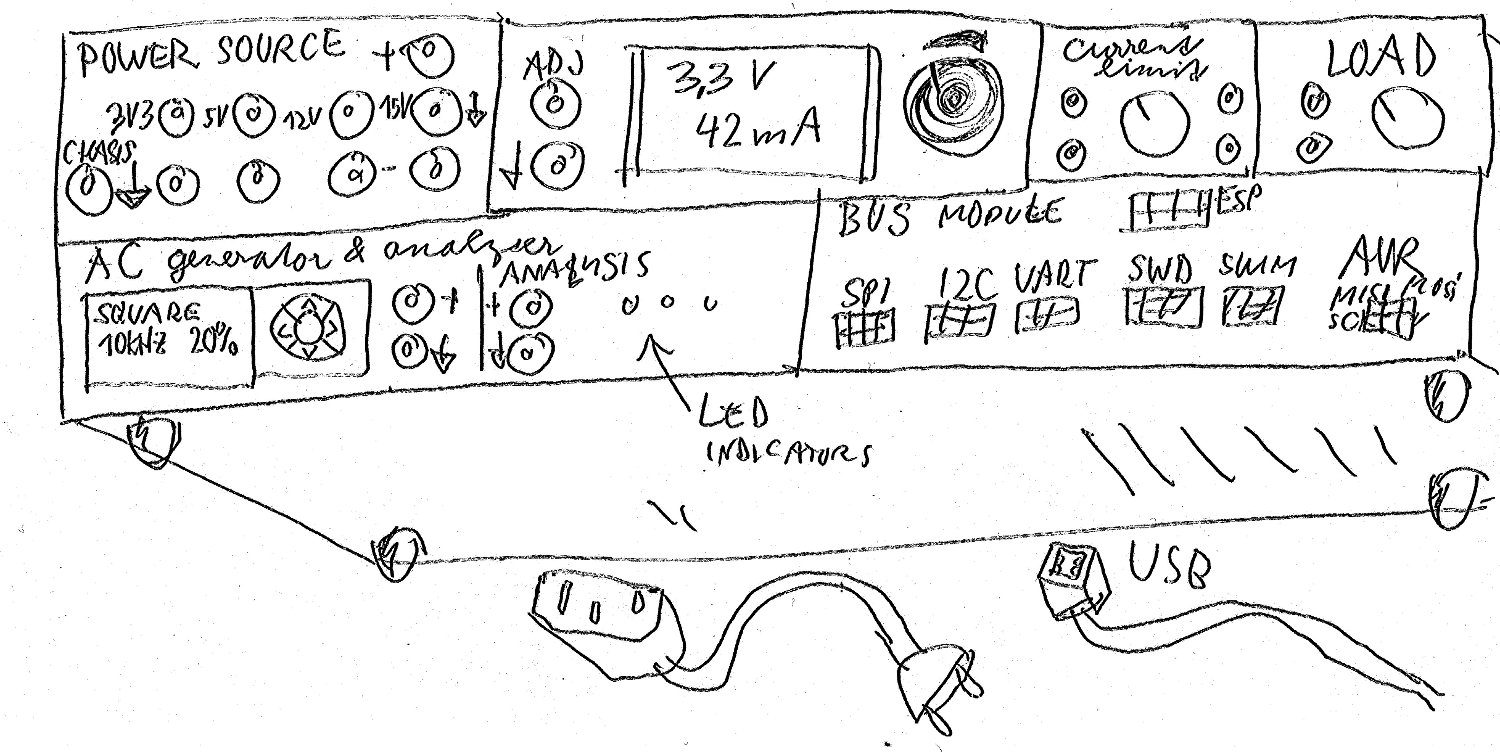
\includegraphics[width=0.7\textwidth] {img/early-sketch.jpg}
	\caption[An early sketch of a universal bench device]{An early (2016) sketch of a universal bench device including a power supply, electronic load, a signal generator and a bus module. The bottom half of the panel is in a large part implemented by GEX.}
\end{figure}
\fi

Building on the experience with earlier embedded projects, an STM32 microcontroller shall be used. Those are ARM Cortex M devices with a wide range of hardware peripherals that appear be a good fit for the project. Low-cost evaluation boards are widely available that could be used as a hardware platform instead of developing a custom \gls{PCB}. Besides, those chips are relatively cheap and already popular in the embedded hardware community; there is a good possibility of the project building a community around it and growing beyond what will be presented in this paper.

\iffalse
Besides the use of existing development boards, custom \glspl{PCB} will be developed in different form factors. The possibilities of wireless connection should be evaluated. This feature should make GEX useful e.g. in mobile robotics or when installed in poorly accessible locations.
\fi







